\documentclass[11pt,a4paper]{article}

% ---- packages ----------------------------------------------------------------
\usepackage[margin=2.5cm]{geometry}
\usepackage{graphicx}
\usepackage{booktabs}
\usepackage{multirow}
\usepackage{amsmath}
\usepackage{hyperref}
\usepackage{caption}
\usepackage{subcaption}
\usepackage{float}
\usepackage{xcolor}
\usepackage{array}
\usepackage{microtype}
\usepackage{parskip}
\usepackage{titlesec}
\usepackage{fancyhdr}
\usepackage{enumitem}

% ---- typography --------------------------------------------------------------
\titleformat{\section}{\large\bfseries}{\thesection}{0.8em}{}
\titleformat{\subsection}{\normalsize\bfseries}{\thesubsection}{0.8em}{}
\setlist[itemize]{leftmargin=1.5em,topsep=2pt,itemsep=1pt}
\captionsetup{font=small, labelfont=bf}
\hypersetup{colorlinks=true, linkcolor=blue!60!black, citecolor=blue!60!black, urlcolor=blue!60!black}

% ---- header / footer ---------------------------------------------------------
\pagestyle{fancy}
\fancyhf{}
\lhead{\small Solid Waste Volume Estimation from Overhead Imagery}
\rhead{\small IIT Bombay}
\cfoot{\thepage}

% ==============================================================================
\begin{document}

\begin{center}
    {\LARGE\bfseries Calibrated Monocular Depth for Solid Waste Volume Estimation\\[0.4em]
    from Overhead Imagery}\\[1.2em]
    {\large Aryan Goyal\textsuperscript{1}}\\[0.4em]
    {\normalsize \textsuperscript{1}IIT Bombay}\\[0.3em]
    {\small \today}
\end{center}

\vspace{0.5em}
\hrule
\vspace{0.8em}

% ==============================================================================
\begin{abstract}
Accurate volumetric estimation of solid waste piles is a practical requirement for waste
management at collection sites, yet conventional approaches rely on manual measurement or
expensive 3-D sensors. This work investigates a low-cost alternative: a single overhead RGB
image captured from a fixed tripod, combined with a monocular metric depth model, to
estimate pile volume. The scene is a 60~cm $\times$ 60~cm collection frame placed on a
flat surface; the camera is mounted 65~cm above the frame floor. Depth maps are produced by
\textit{DepthAnythingV2-Metric-Indoor-Large} and converted to height maps through floor-plane
fitting. A scene-specific calibration factor, derived from a small set of ground-truth labelled
captures, corrects for systematic depth compression and material fluffing. Evaluated on
mixed-composition waste piles (plastic, paper, cardboard, metal cans, and single-use
wrappers) at three mass levels (670~g, 480~g, and 660~g net), the calibrated system
achieves volumetric errors of 2.8\% and 7.8\% on two of the three conditions, with 100\%
depth-sanity verification across all captures. These results demonstrate that monocular depth,
combined with a simple one-parameter calibration, is a viable pathway toward practical
in-situ waste volume estimation.
\end{abstract}

\vspace{0.5em}
\hrule
\vspace{1em}

% ==============================================================================
\tableofcontents
\newpage

% ==============================================================================
\section{Introduction}



The central idea explored here is to combine a fixed overhead camera with a monocular metric
depth network. Given a known scene footprint (the floor area enclosed by the containment
frame), and an estimate of each pixel's height above the floor, volume is simply the integral
of the height map over that footprint. The challenge is that monocular depth models are
calibrated to indoor scenes at typical human-viewing distances; at very close range (65~cm
camera-to-floor), the relative depth span of a 20~cm pile is compressed to a small fraction
of the model's output range. A per-scene calibration factor bridges this gap.

This report describes the dataset collected at IIT Bombay, the volume estimation pipeline,
the calibration procedure, and results across multiple pile conditions.

% ==============================================================================
\section{Dataset}
\label{sec:dataset}

\subsection{Acquisition Setup}

Images were collected at the IIT Bombay solid waste site using an iPhone camera
mounted on a fixed overhead height. The containment frame is a white-chalked box with
an interior footprint of $60~\text{cm} \times 60~\text{cm}$ (area = 0.36~m$^2$). The camera
lens is positioned approximately 65~cm above the floor of the frame, oriented vertically
downward. At this height the box frame fills the vast majority of the image, providing a
natural scene boundary and a stable reference geometry.

Figure~\ref{fig:site} shows the collection site.

\begin{figure}[H]
    \centering
    \begin{subfigure}[b]{0.48\textwidth}
        \centering
        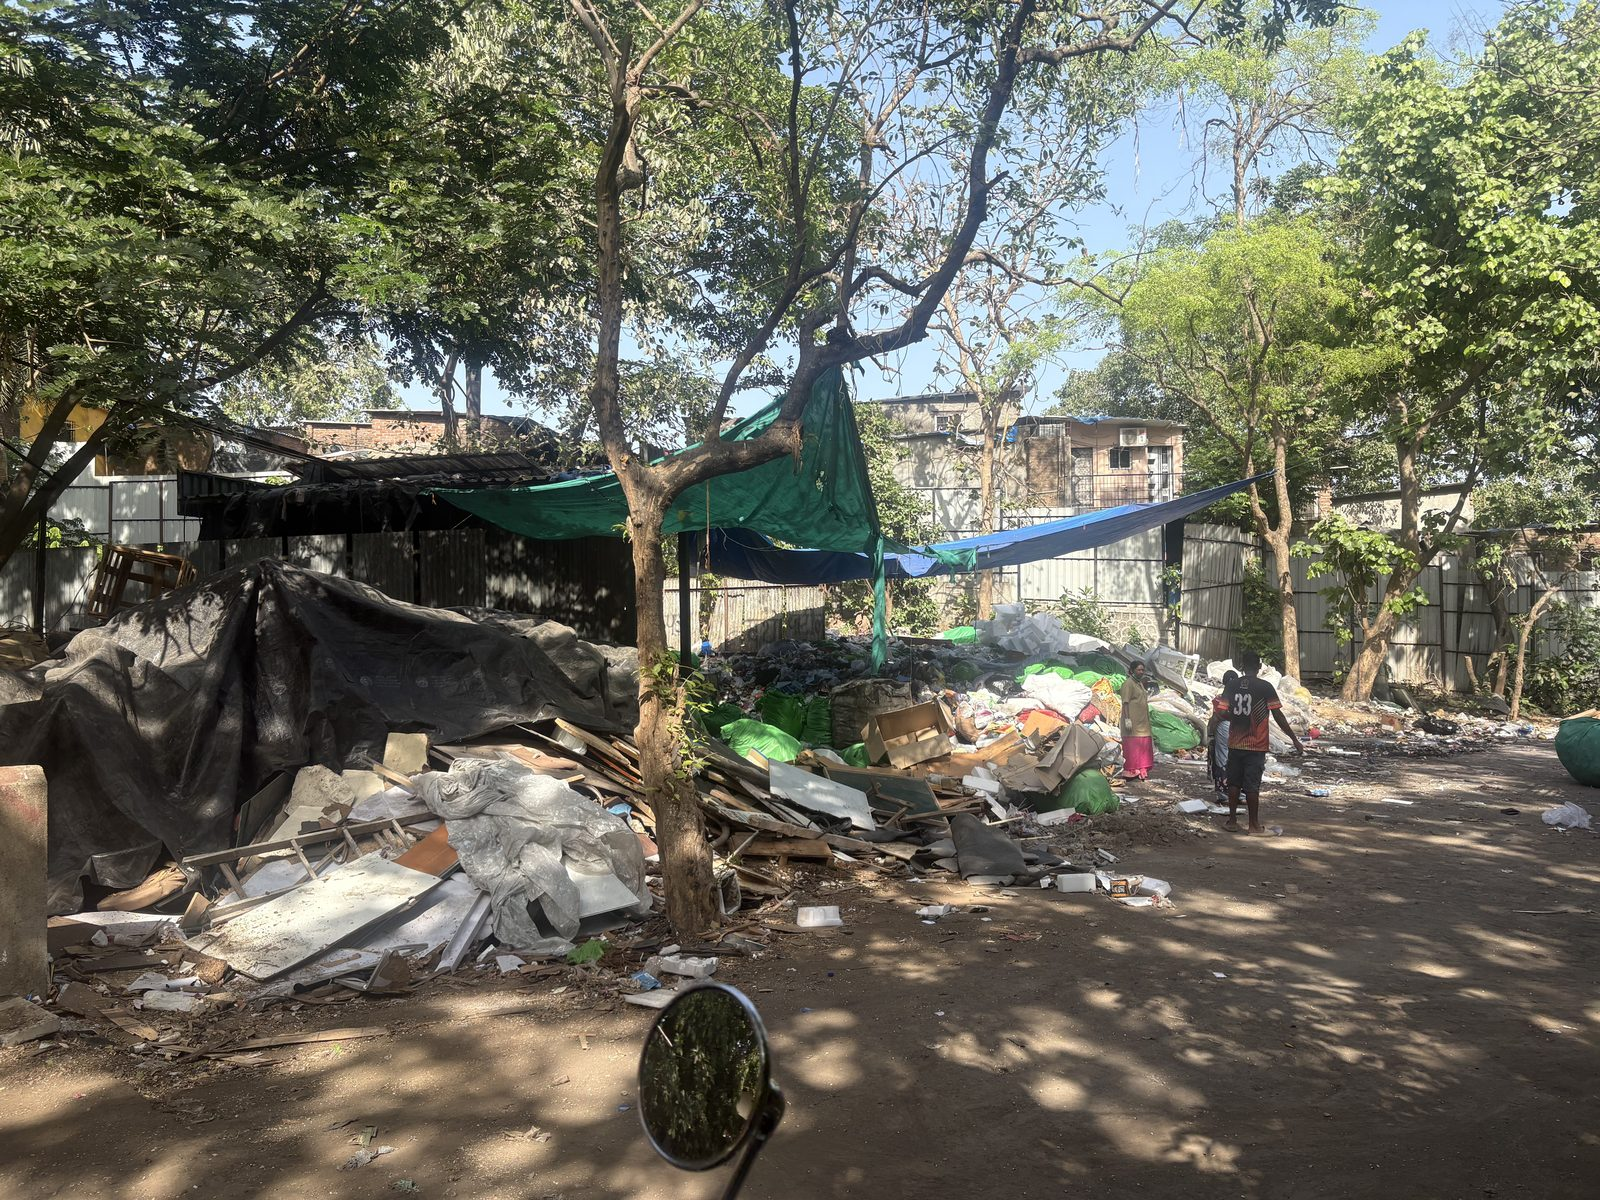
\includegraphics[width=\linewidth]{images/site_setup.jpg}
        \caption{Collection site overview.}
    \end{subfigure}
    \hfill
    \begin{subfigure}[b]{0.48\textwidth}
        \centering
        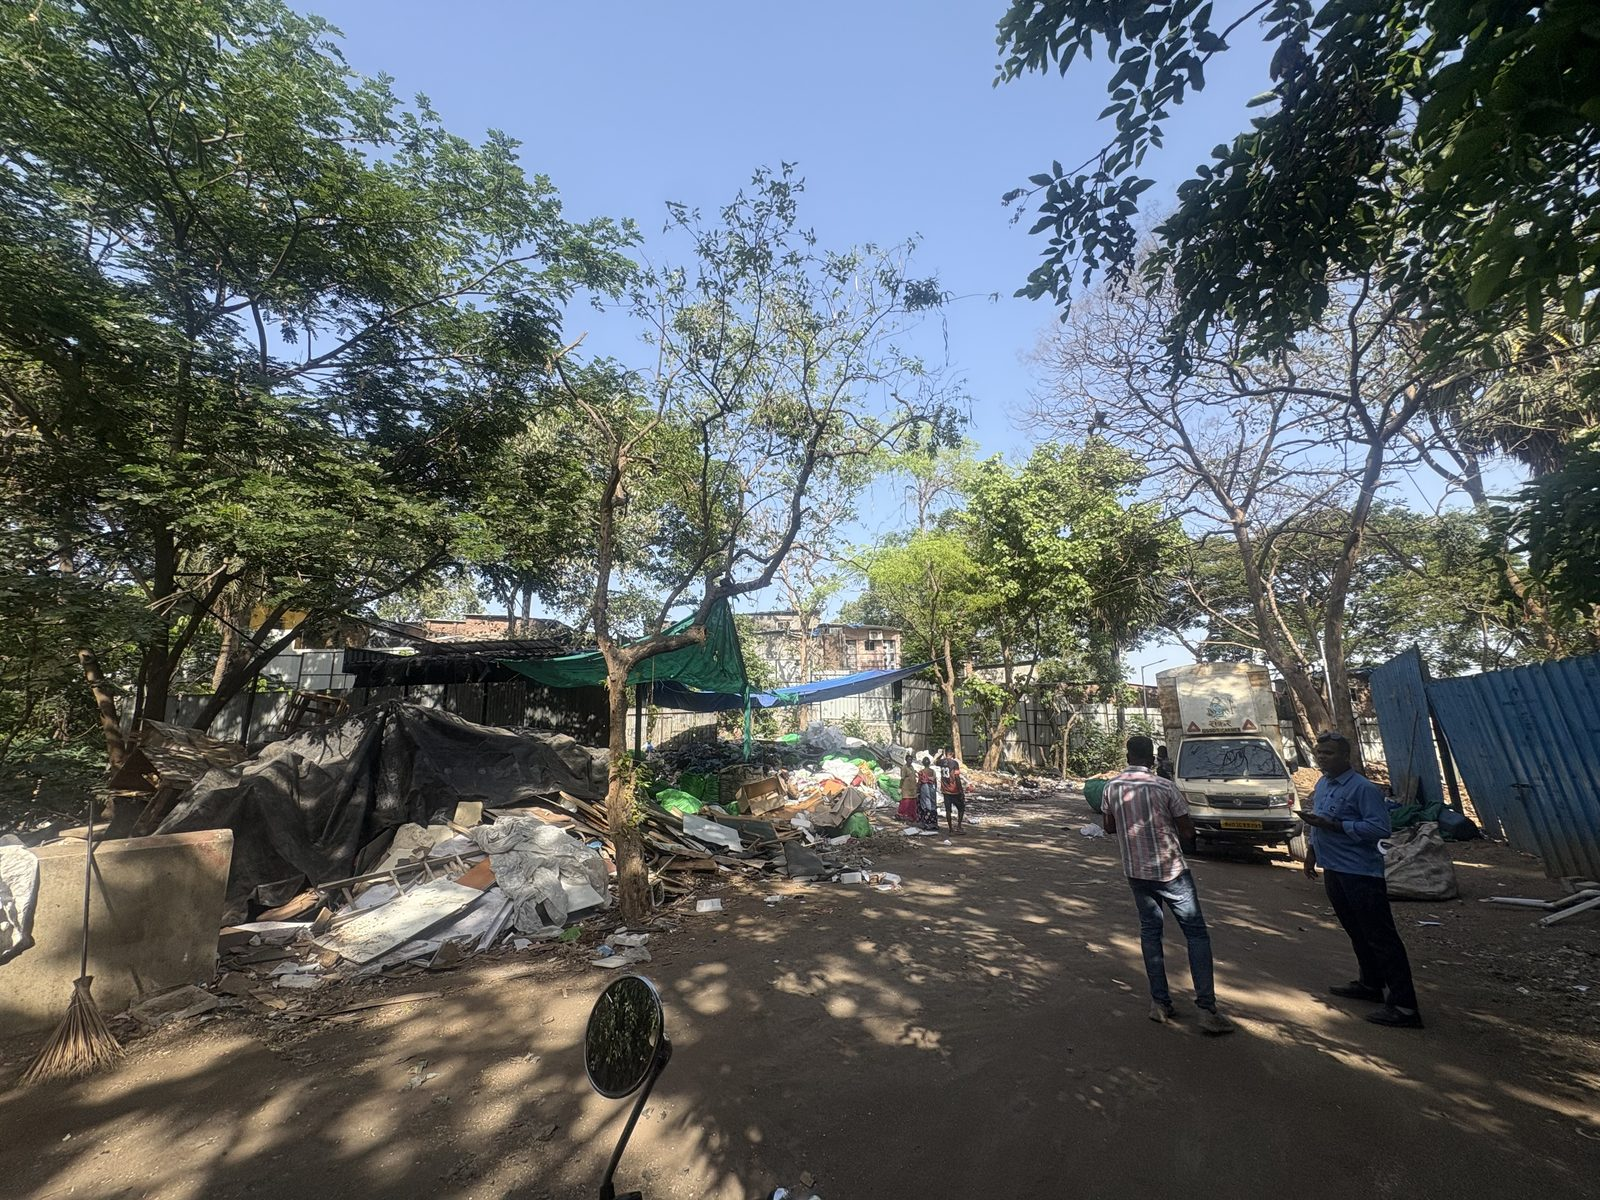
\includegraphics[width=\linewidth]{images/site_setup2.jpg}
        \caption{Collection site overview 2.}
    \end{subfigure}
    \caption{IIT Bombay solid waste collection site. The 60~cm $\times$ 60~cm white containment
    frame serves as the scene reference. The camera tripod positions the lens 65~cm directly
    above the frame floor.}
    \label{fig:site}
\end{figure}

\subsection{Pile Conditions}

Three mass conditions of \textit{mixed solid waste} were studied. The waste comprised a
realistic mix of materials: plastic bottles and bags, paper, cardboard, metal cans, and
single-use food/beverage wrappers. Masses below are net (gross minus 270~g tare).

\begin{center}
\renewcommand{\arraystretch}{1.3}
\begin{tabular}{@{}clcc@{}}
\toprule
\textbf{Condition} & \textbf{Material} & \textbf{Net Mass (g)} & \textbf{Geometric GT volume (L)} \\
\midrule
Pile A & Mixed (plastic, paper, cardboard, cans, wrappers) & 670 & 18.0 \\
Pile B & Mixed (plastic, paper, cardboard, cans, wrappers) & 480 & 18.0 \\
Pile C & Mixed (plastic, paper, cardboard, cans, wrappers) & 660 & 18.0 \\
\bottomrule
\end{tabular}
\end{center}

The ground-truth (GT) volume was obtained by manual geometric measurement of the pile's
approximate bounding box (20~cm height $\times$ 30~cm $\times$ 30~cm footprint = 18~L).
This method yields a \emph{geometric} volume that is a conservative lower bound; the actual
bulk volume of the loosely arranged material can be larger due to air pockets between pieces,
a phenomenon referred to as material \textit{fluffing}. The calibration procedure accounts
for this systematically.

For each pile condition, a series of overhead photographs was captured from slightly varying
viewpoints: the camera tripod was repositioned within a small radius around the vertical axis,
and captures were taken across different pile arrangements and ambient lighting conditions.
This multi-view protocol provides a distribution of raw depth-based volume estimates for
each pile, from which a robust calibration factor can be derived.

Figure~\ref{fig:samples} shows representative captures for pile conditions.

\begin{figure}[H]
    \centering
    \begin{subfigure}[b]{0.32\textwidth}
        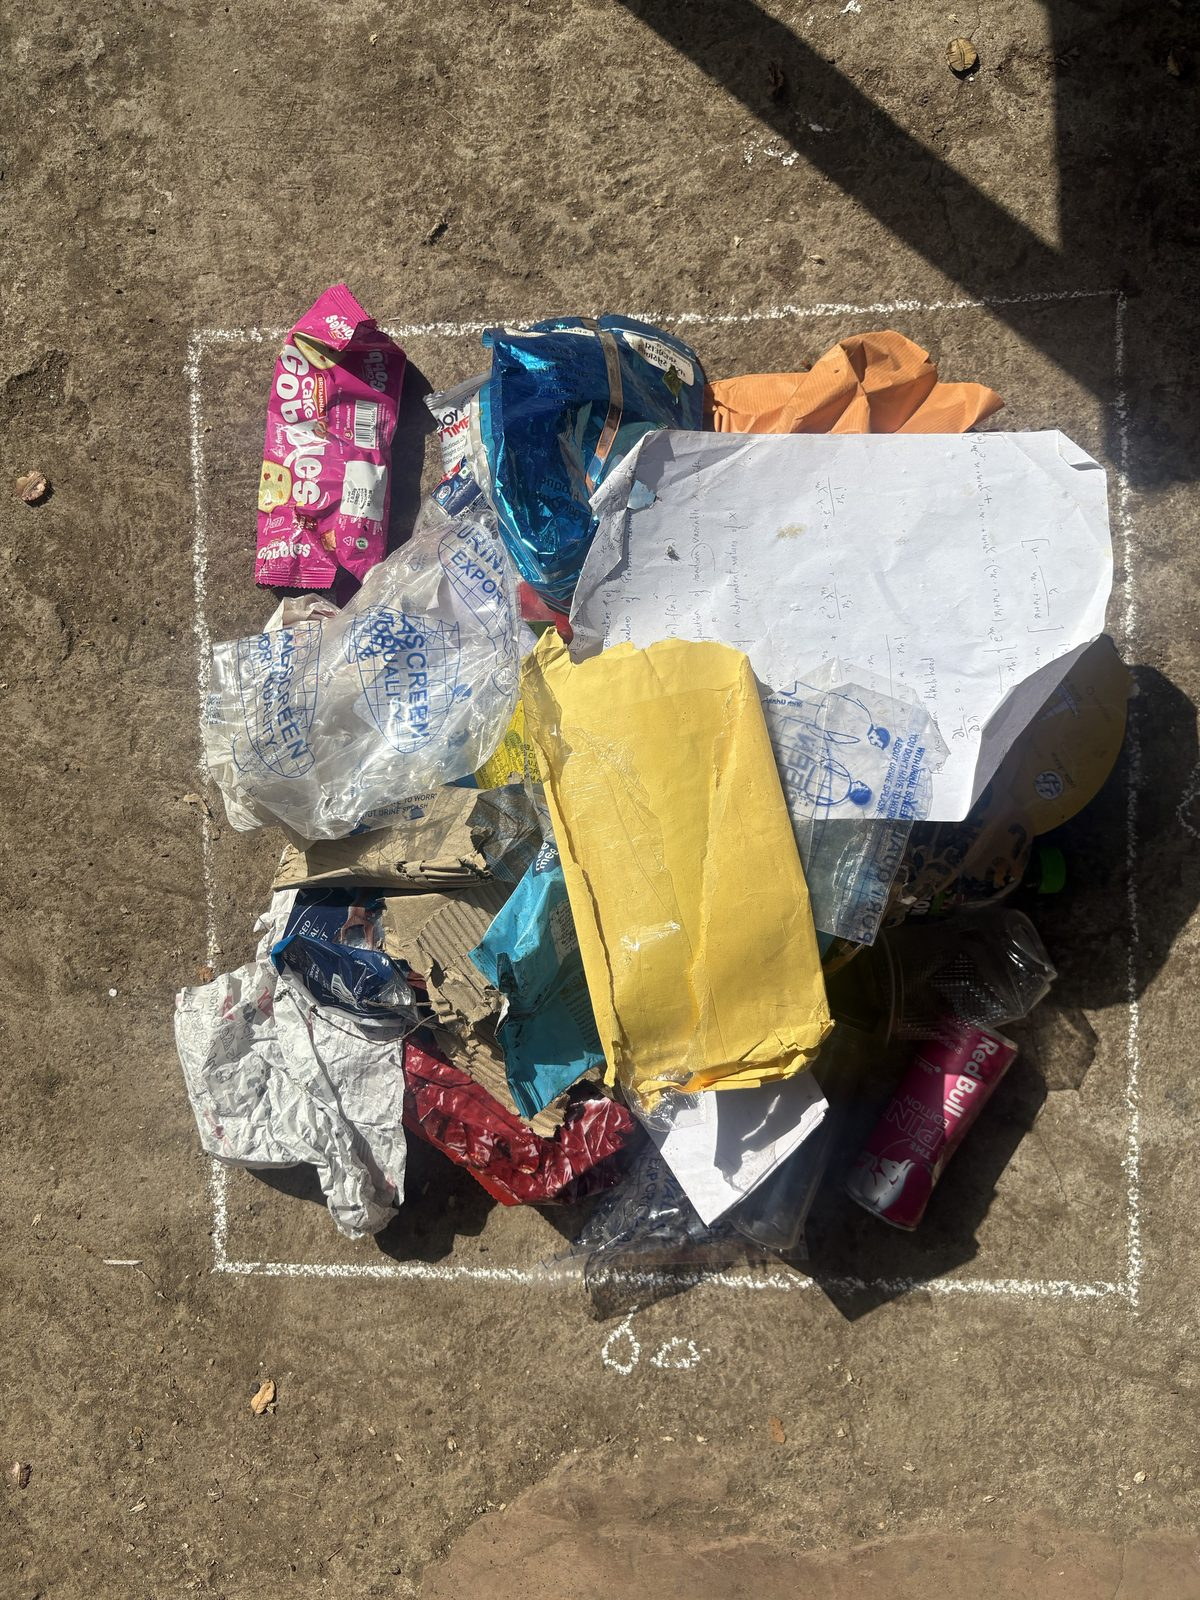
\includegraphics[width=\linewidth]{images/pile1_sample.jpg}
        \caption{Pile A (670~g net)}
    \end{subfigure}
    \hfill
    \begin{subfigure}[b]{0.32\textwidth}
        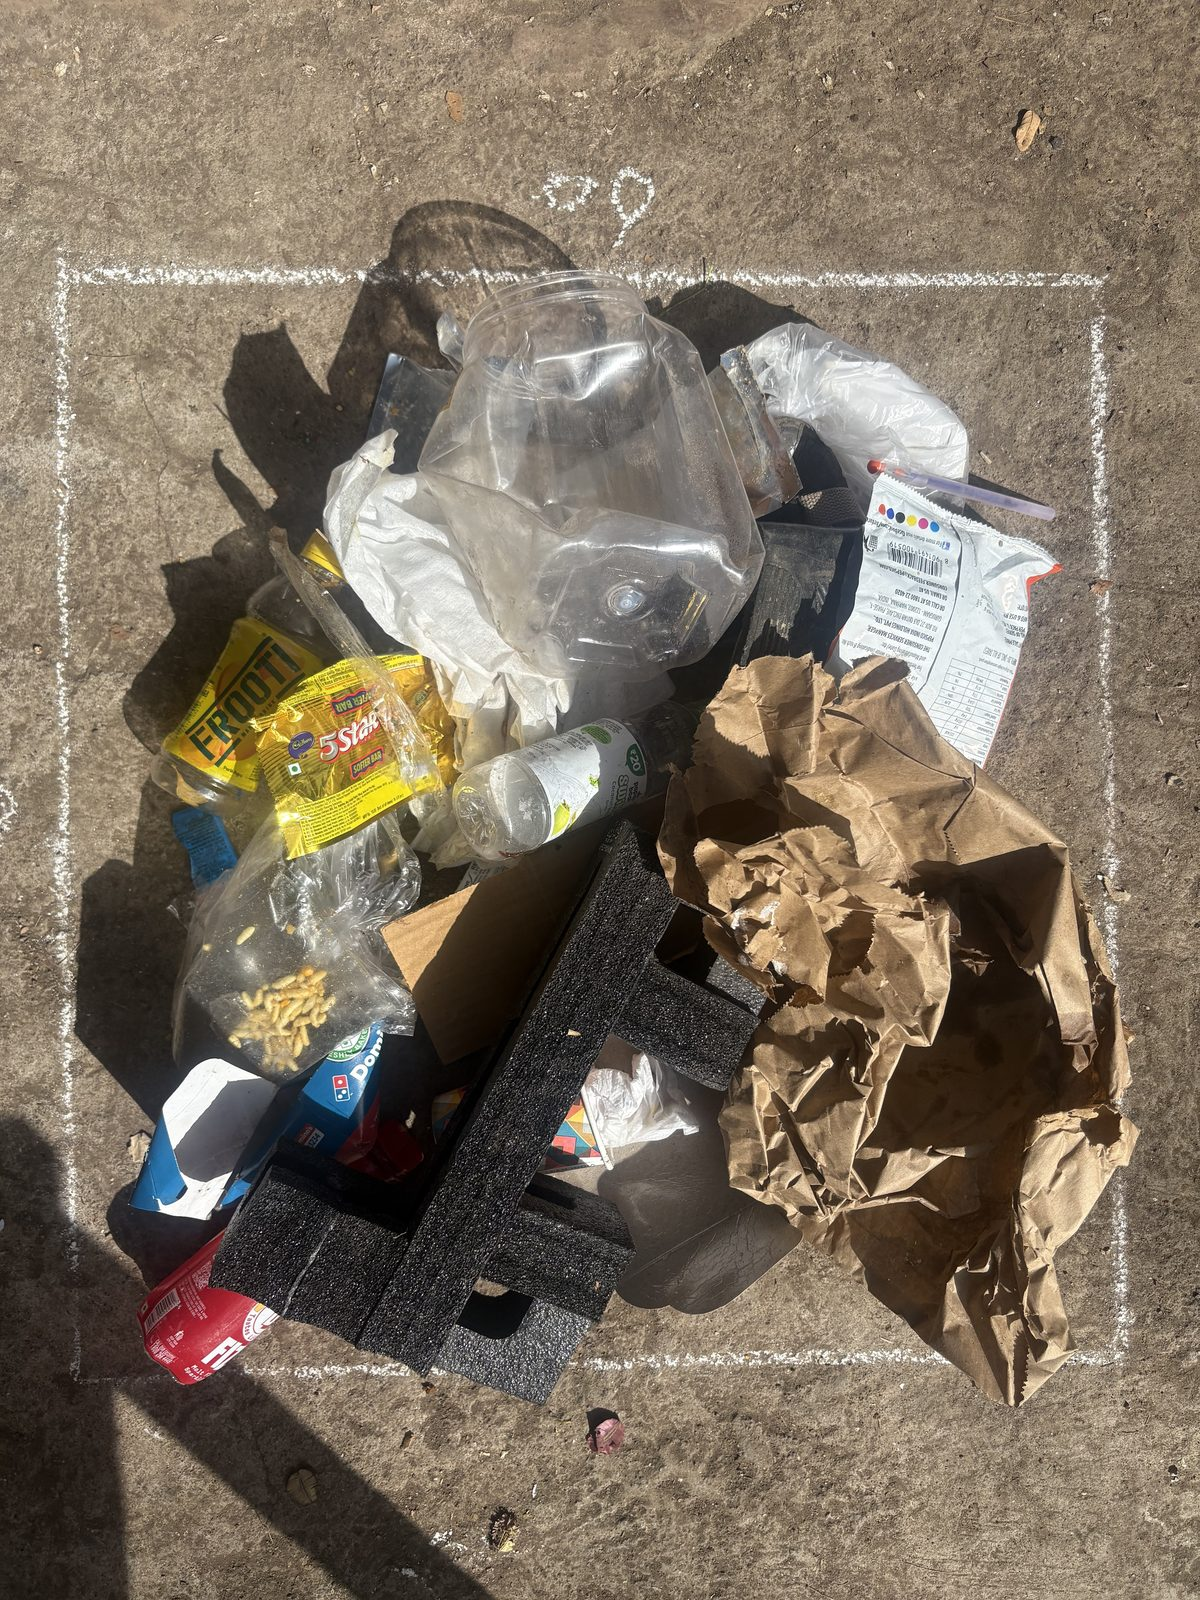
\includegraphics[width=\linewidth]{images/pile2_sample.jpg}
        \caption{Pile B (480~g net)}
    \end{subfigure}
    \hfill
    \begin{subfigure}[b]{0.32\textwidth}
        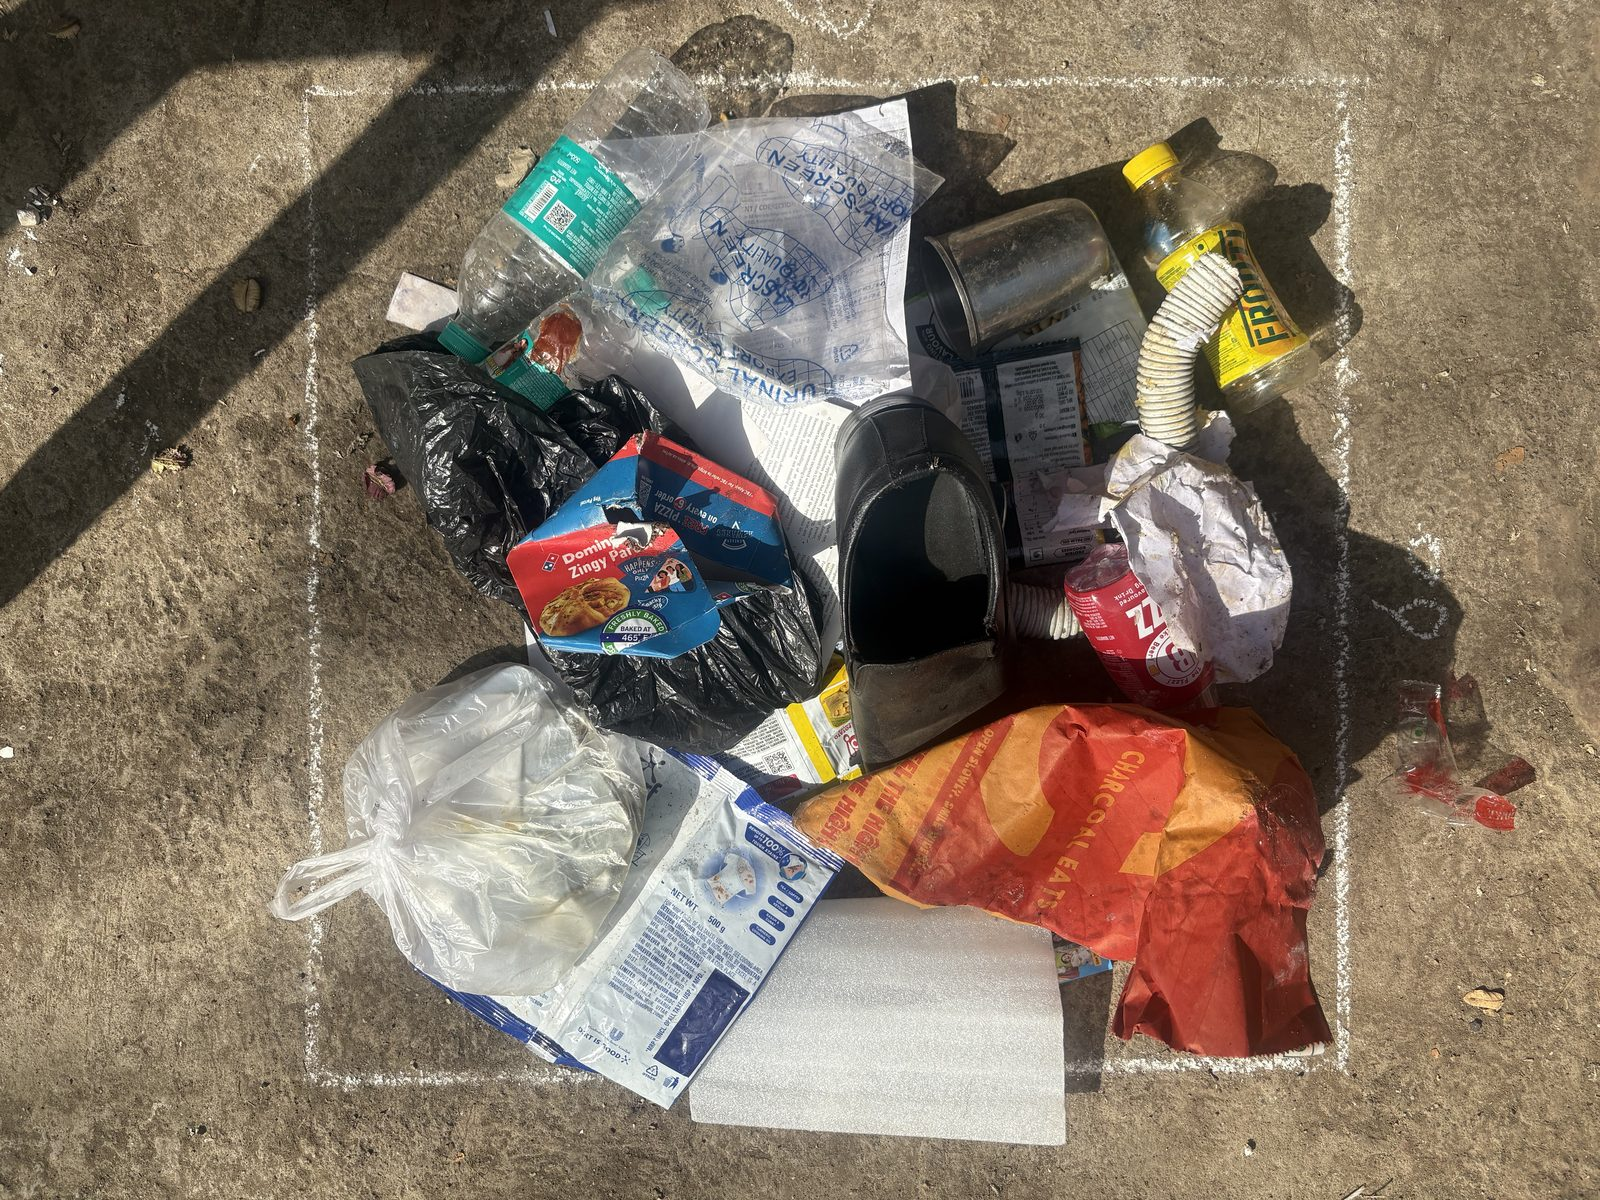
\includegraphics[width=\linewidth]{images/pile3_sample.jpg}
        \caption{Pile C (660~g net)}
    \end{subfigure}
    \caption{Representative overhead captures for each pile condition. The white containment
    frame is visible at the image periphery. Pile volume increases with mass; differences in
    pile spread and height are visible across conditions.}
    \label{fig:samples}
\end{figure}

\begin{figure}[H]
    \centering
    \begin{subfigure}[b]{0.32\textwidth}
        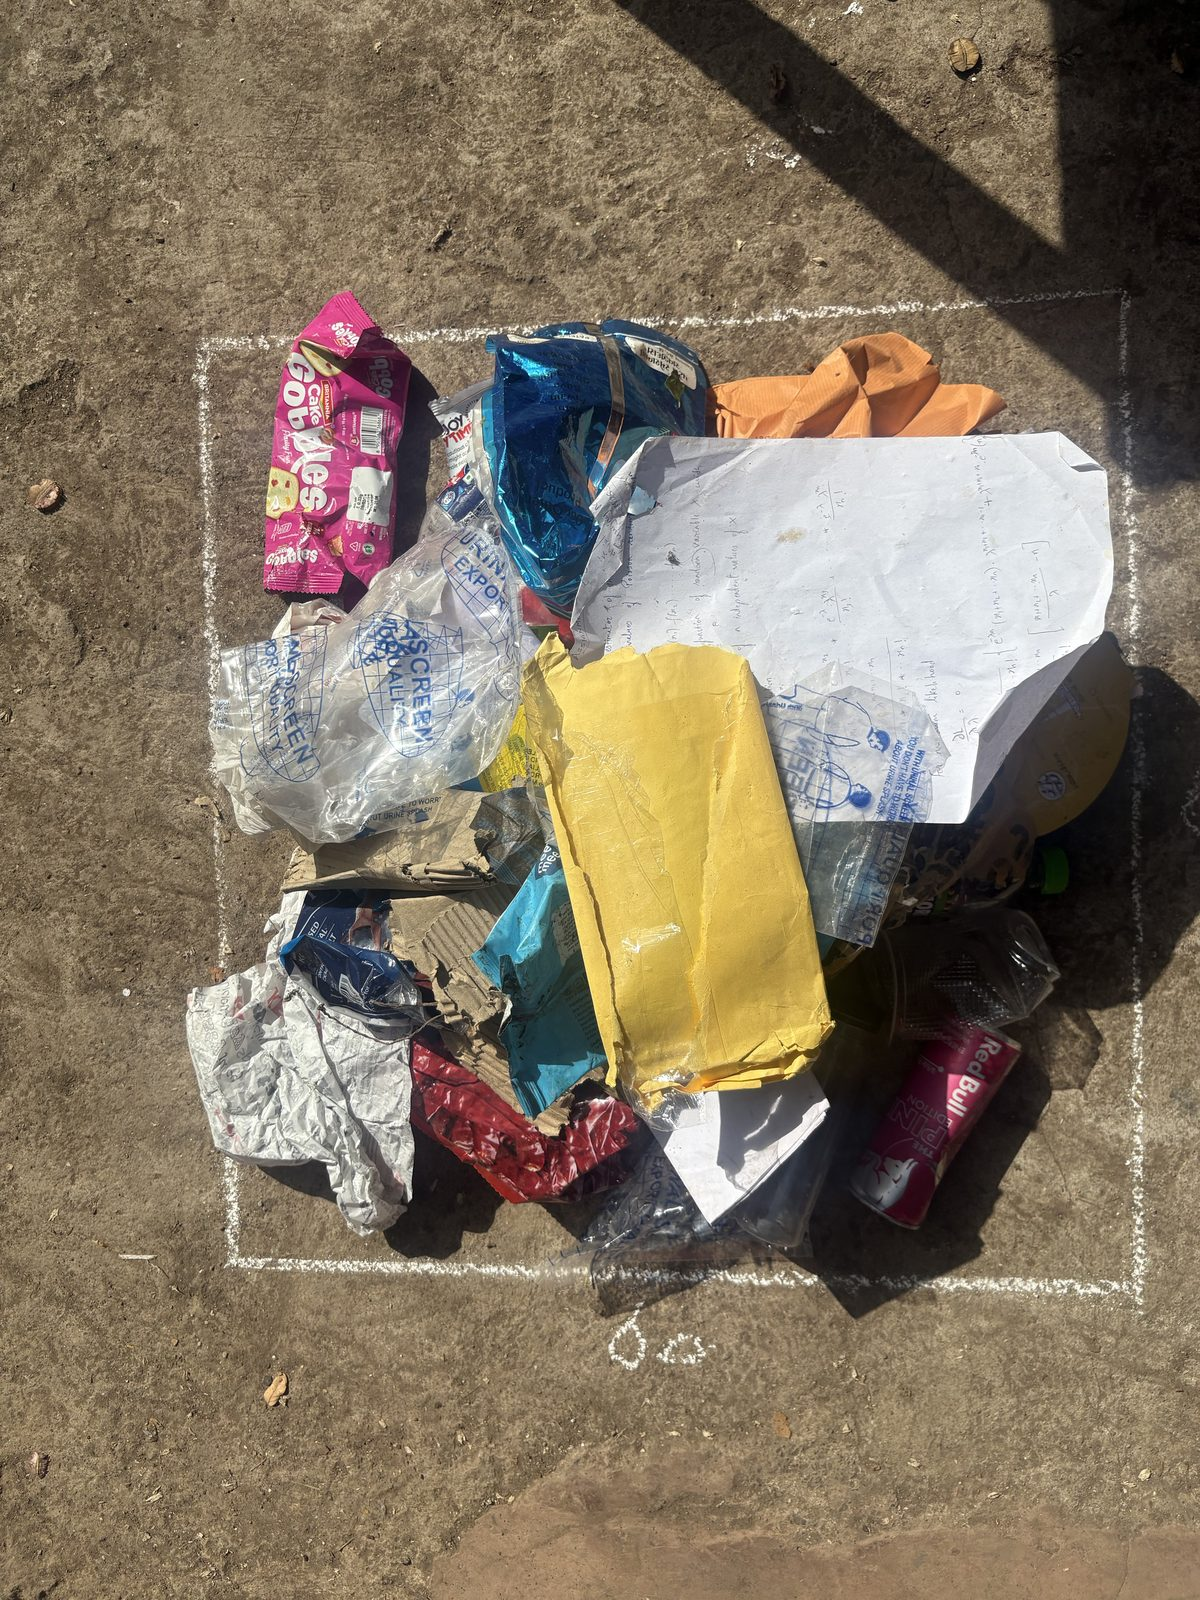
\includegraphics[width=\linewidth]{images/pile1_sample2.jpg}
        \caption{Pile A, alternate view}
    \end{subfigure}
    \hfill
    \begin{subfigure}[b]{0.32\textwidth}
        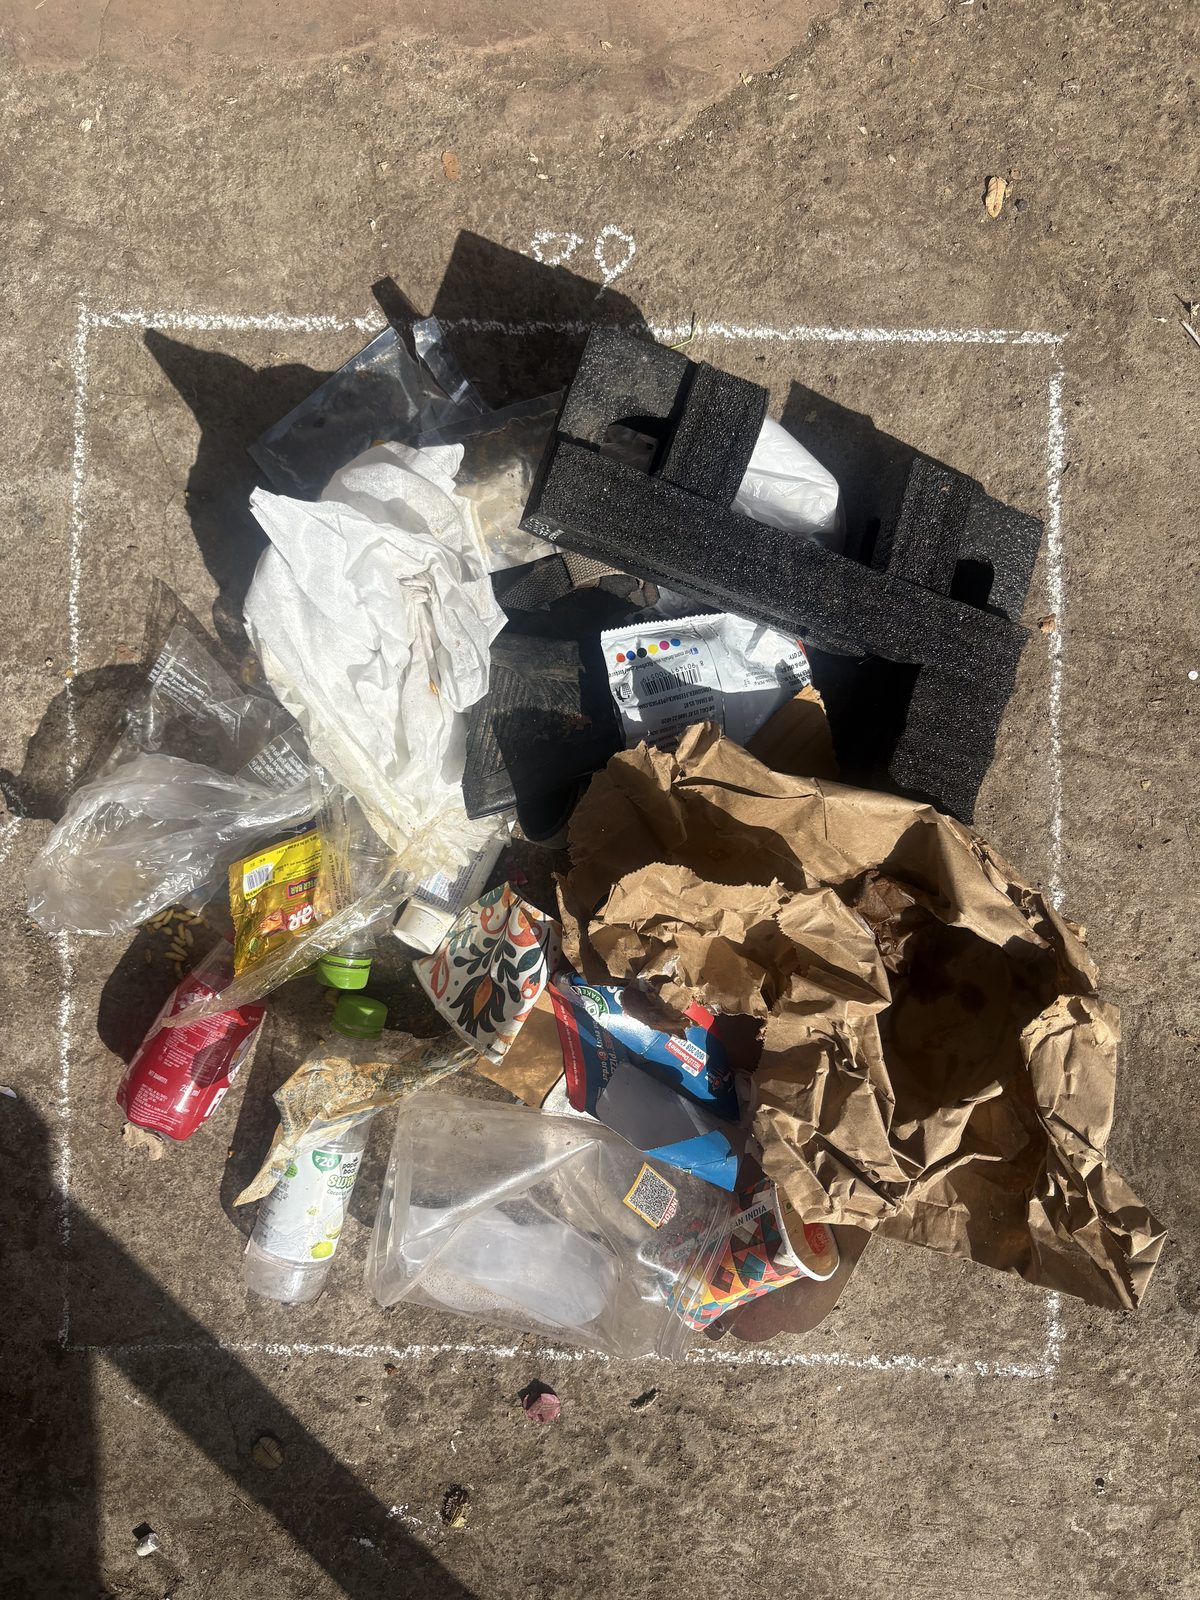
\includegraphics[width=\linewidth]{images/pile2_sample2.jpg}
        \caption{Pile B, alternate view}
    \end{subfigure}
    \hfill
    \begin{subfigure}[b]{0.32\textwidth}
        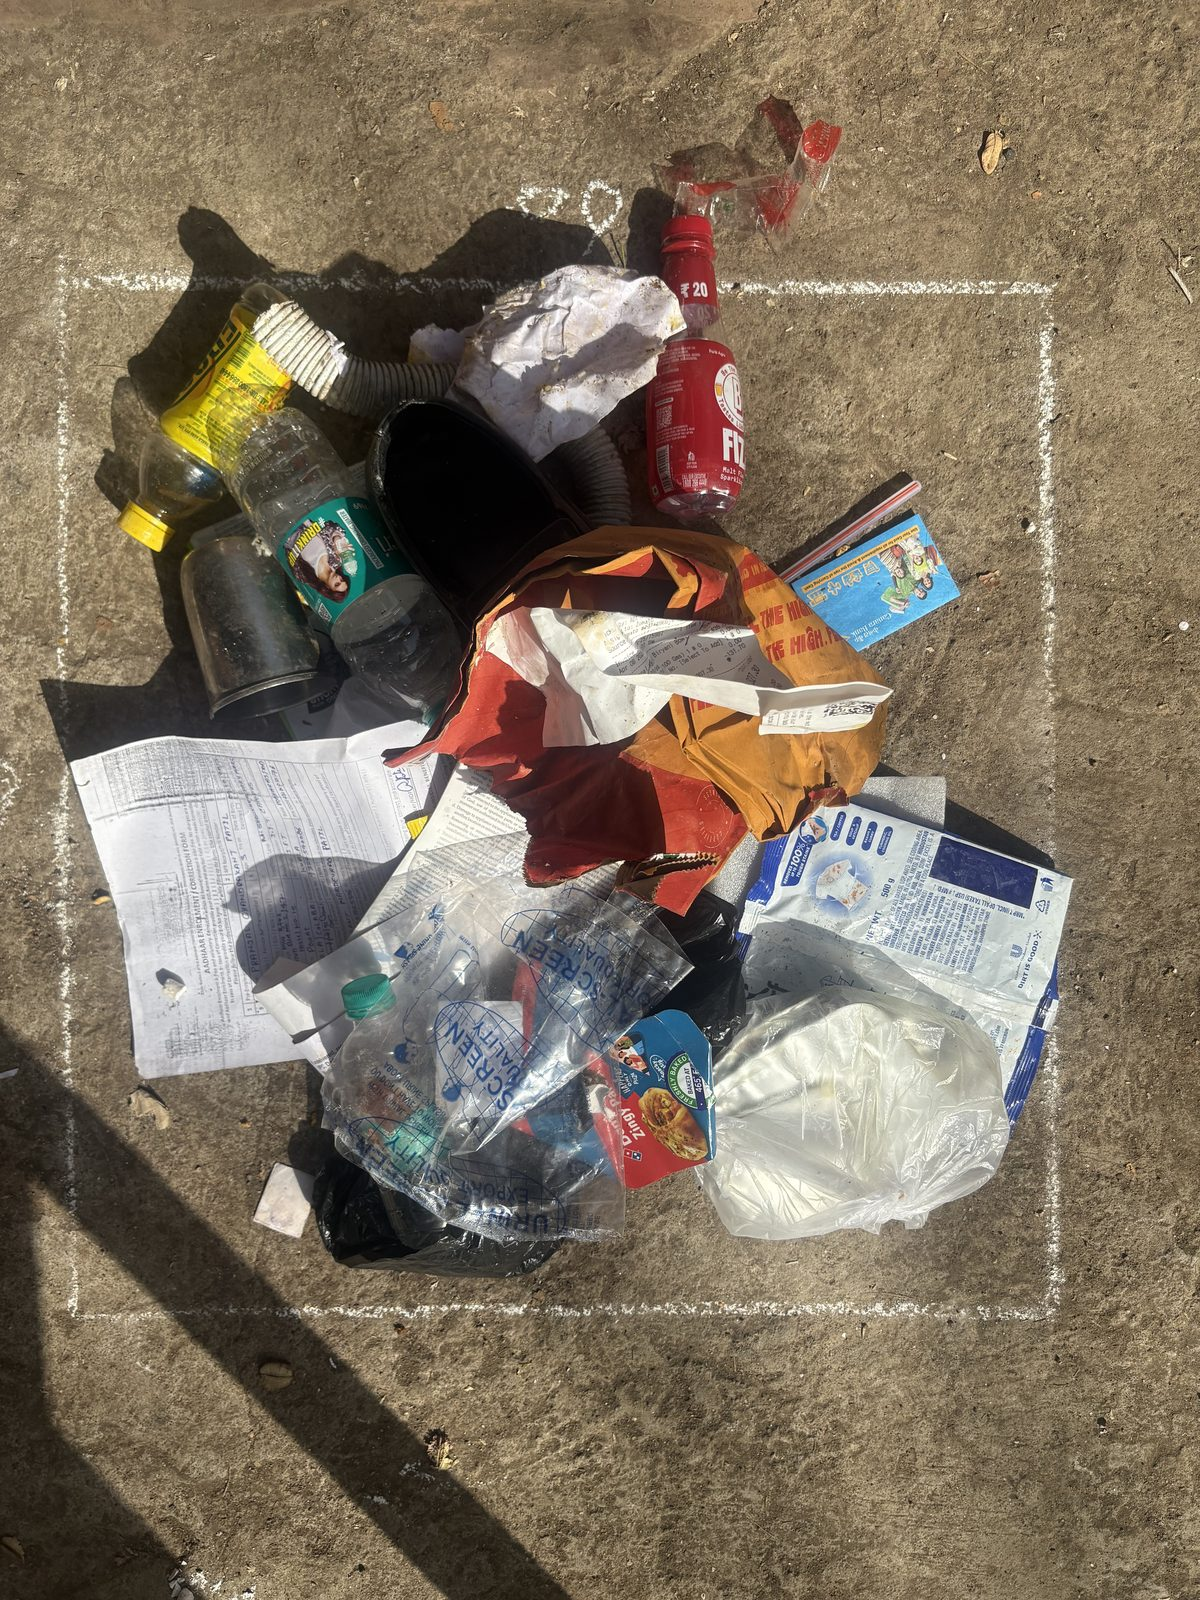
\includegraphics[width=\linewidth]{images/pile3_sample2.jpg}
        \caption{Pile C, alternate view}
    \end{subfigure}
    \caption{Additional representative captures showing variation in pile arrangement and
    viewpoint across the data collection protocol.}
    \label{fig:samples2}
\end{figure}

\subsection{Data Split}

For each pile condition, the captured images were divided into a \textbf{calibration partition}
and an \textbf{evaluation partition}. The calibration partition provides the GT-labelled images
used to derive the calibration factor (described in Section~\ref{sec:calibration}). The evaluation
partition contains held-out images to which the derived factor is then applied blindly, simulating
deployment on unseen captures from the same scene type.

% ==============================================================================
\section{Methodology}
\label{sec:method}

The volume estimation pipeline consists of four stages: depth inference, floor-plane fitting,
height-map computation, and volume integration. A single-parameter calibration factor is
then applied to the integrated volume.

\subsection{Depth Inference with DepthAnythingV2}

The depth model used is \textbf{DepthAnythingV2-Metric-Indoor-Large}~\cite{depth_anything_v2},
a transformer-based monocular depth estimator fine-tuned for metric (absolute) depth prediction
in indoor environments. Unlike relative depth models, DepthAnythingV2-Metric produces depth
values in metres, enabling direct conversion to physical heights without additional scale recovery.

The model takes a full-resolution RGB image as input and returns a single-channel depth map
of the same spatial dimensions. All inference is performed on a single GPU with mixed-precision
computation. At the operating distance of 65~cm, the model typically outputs floor depths in
the range of 1.75~m to 2.25~m (due to the model's indoor calibration, raw depths do not
correspond to the physical 65~cm; this systematic offset is handled in the floor-fitting stage).

\subsection{Floor-Plane Fitting}

The floor of the containment frame acts as the depth reference surface. Because the camera
can have a slight non-vertical tilt, a planar floor model is fitted rather than assuming a
constant floor depth. The procedure is:

\begin{enumerate}
    \item Identify \textbf{floor candidate pixels}: the deepest 1\% of valid depth values.
    At 65~cm camera height with the frame filling the image, these pixels correspond to the
    frame edges and corners where no pile material is present.
    \item Fit a \textbf{tilted plane} to the $(x, y, d)$ coordinates of the floor candidates
    using least-squares regression, where $d$ is the raw depth value and $(x, y)$ are pixel
    coordinates.
    \item Evaluate the fitted plane at every pixel to obtain a \textbf{predicted floor depth}
    $\hat{d}_\text{floor}(x, y)$.
    \item Derive a \textbf{depth-to-height scale factor} $s$ by requiring that the median floor
    depth corresponds to the known physical camera height $H = 0.65$~m:
    \[
        s = \frac{H}{\tilde{d}_\text{floor}}
    \]
    where $\tilde{d}_\text{floor}$ is the median of the fitted floor values.
\end{enumerate}

\subsection{Height Map Computation}

For each pixel $(i,j)$, the pile height above the local floor is:
\[
    h(i,j) = \bigl(\hat{d}_\text{floor}(i,j) - d(i,j)\bigr) \times s
\]

where $d(i,j)$ is the raw model depth at that pixel. Pixels where $d$ exceeds the local
floor estimate (i.e., they are below the floor) are clipped to zero. A fixed minimum height
threshold of 1~cm is applied to suppress noise in regions containing no pile material:
\[
    h_\text{clean}(i,j) = \max\bigl(h(i,j) - 0.01,\ 0\bigr)
\]

\subsection{Depth Sanity Check}

Before accepting a height map, a geometric sanity check is applied: the mean depth in the
central 70\% of the image should be \textit{smaller} (closer to the camera) than the mean
depth of the 15\% border strip. This checks that the model has correctly recognised the pile
as elevated above the floor. In all captures evaluated in this study, this sanity check passes,
confirming that DepthAnythingV2 reliably detects the pile geometry in this setup.

\subsection{Volume Integration}

Given the height map $h_\text{clean}$, the volume is obtained by summing pixel heights and
multiplying by the physical area per pixel:

\[
    V_\text{raw} = \sum_{i,j} h_\text{clean}(i,j) \times A_\text{px}
    \quad \text{where} \quad
    A_\text{px} = \frac{A_\text{box}}{N_\text{px}} = \frac{0.36~\text{m}^2}{W \times H}
\]

and $W$, $H$ are the image width and height in pixels. The result is converted from cubic
metres to litres ($\times 1000$).

\subsection{Calibration Factor Derivation}
\label{sec:calibration}

The raw volume $V_\text{raw}$ systematically underestimates or overestimates the true pile
volume for two reasons:

\begin{itemize}
    \item \textbf{Depth compression}: at very close range (65~cm), the model's relative depth
    span is compressed relative to the physical height difference. The depth scale factor $s$
    partially corrects for this, but a residual model bias remains.
    \item \textbf{Material fluffing}: the geometric GT volume (18~L) is measured on a settled
    bounding box, but the actual bulk volume of the arranged pile can differ due to inter-piece
    air pockets.
\end{itemize}

To account for both effects with a single correction, a per-condition \textbf{calibration
factor} CF is computed from the calibration partition:
\[
    \text{CF} = \frac{V_\text{GT}}{\overline{V}_\text{raw,\,cal}}
\]

where $\overline{V}_\text{raw,\,cal}$ is the mean raw predicted volume across calibration
images. This CF is then applied to all evaluation-partition images of the same pile condition
to produce the final estimate:
\[
    V_\text{est} = \text{CF} \times V_\text{raw}
\]

% ==============================================================================
\section{Results}
\label{sec:results}

\subsection{Depth Map Visualisation}

Figure~\ref{fig:vis} shows the three-panel depth visualisation produced for a representative
image from each pile condition: the original RGB frame, the raw depth map from
DepthAnythingV2 (brighter = closer to camera), and the calibrated height heatmap overlaid on
the RGB image (warmer colours = greater pile height). The depth maps show a clear central
elevation corresponding to the pile, surrounded by the flat frame floor at the image periphery,
confirming that the model is detecting pile geometry correctly.

\begin{figure}[H]
    \centering
    \begin{subfigure}[b]{\textwidth}
        \centering
        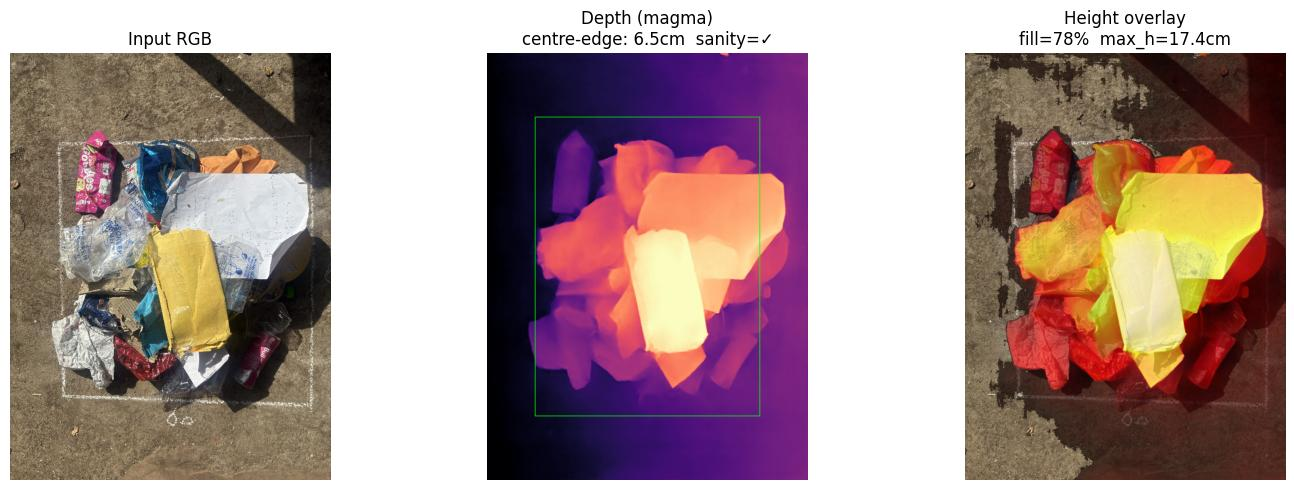
\includegraphics[width=0.95\linewidth]{images/pile1_vis.jpg}
        \caption{Pile A (670~g net): raw depth map and height overlay.}
    \end{subfigure}\\[0.8em]
    \begin{subfigure}[b]{\textwidth}
        \centering
        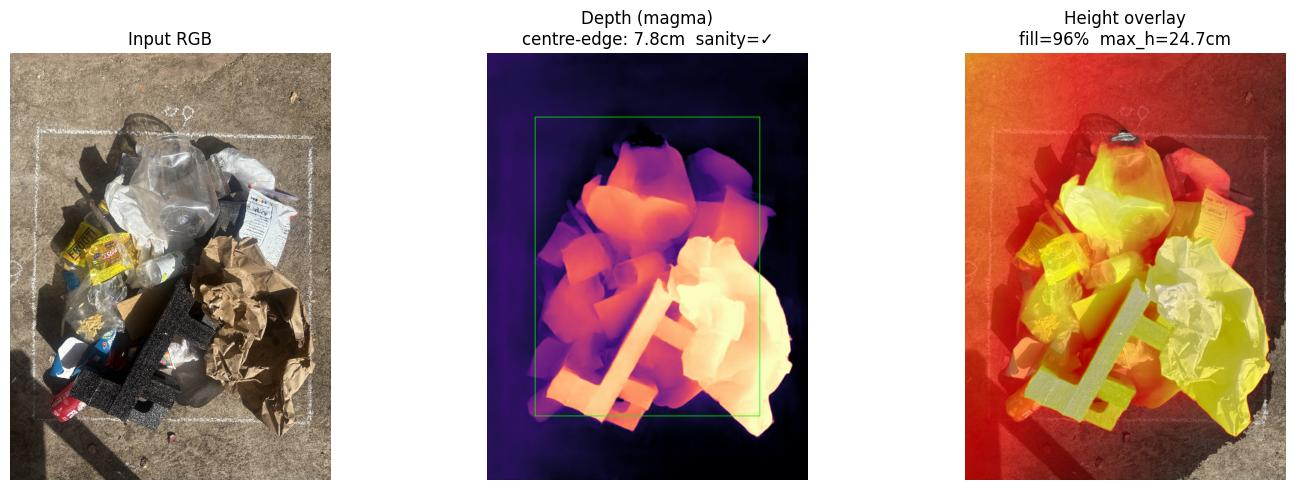
\includegraphics[width=0.95\linewidth]{images/pile2_vis.jpg}
        \caption{Pile B (480~g net): raw depth map and height overlay.}
    \end{subfigure}\\[0.8em]
    \begin{subfigure}[b]{\textwidth}
        \centering
        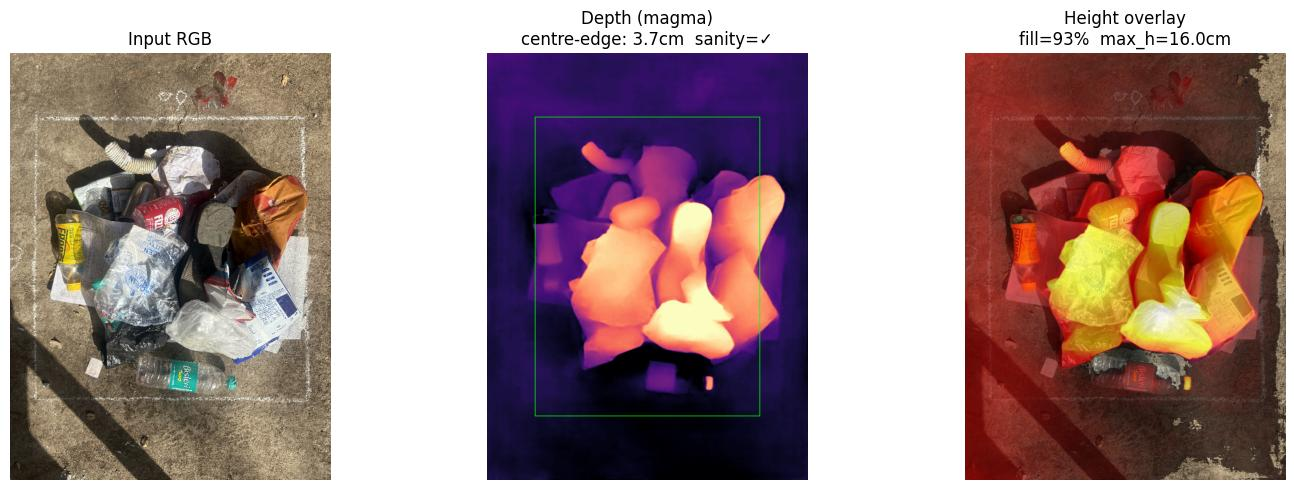
\includegraphics[width=0.95\linewidth]{images/pile3_vis.jpg}
        \caption{Pile C (660~g net): raw depth map and height overlay.}
    \end{subfigure}
    \caption{Three-panel depth visualisation for representative captures. Left: original RGB
    image. Centre: DepthAnythingV2 depth map (brighter pixels are closer to the camera, i.e.\
    taller pile material). Right: height heatmap overlaid on RGB (jet colormap; red = highest).
    The green rectangle in the depth panel marks the central region used in the sanity check.}
    \label{fig:vis}
\end{figure}

\subsection{Pile-Level Volume Estimates and Calibration Factors}

Table~\ref{tab:results} summarises the raw predicted volume, derived calibration factor, and
final calibrated volume for each pile condition. The CF is derived from the calibration partition
and then applied to the held-out evaluation images. Figure~\ref{fig:chart} plots the distribution
of raw predicted volumes across all captures alongside the GT line.

\begin{table}[H]
\centering
\caption{Volume estimation results per pile condition. CF is the calibration factor derived
from the calibration partition. Calibrated volume = CF $\times$ mean raw predicted volume.
Error is against the geometric GT of 18~L.}
\label{tab:results}
\renewcommand{\arraystretch}{1.4}
\resizebox{\linewidth}{!}{%
\begin{tabular}{@{}lccccccc@{}}
\toprule
\textbf{Pile} & \textbf{Mass (g)} & \textbf{GT (L)} & \textbf{Raw Mean (L)} & \textbf{Raw Std (L)}
    & \textbf{CF} & \textbf{Cal.\ Vol.\ (L)} & \textbf{Error (\%)} \\
\midrule
Pile A & 670 & 18.0 & 13.4 & 2.1 & 1.38 & 18.5 & 2.8 \\
Pile B & 480 & 18.0 & 37.8 & 17.7 & 0.48 & 18.1 & 0.6 \\
Pile C & 660 & 18.0 & 19.0 & 5.4 & 1.02 & 19.4 & 7.8 \\
\midrule
\multicolumn{6}{l}{\textit{Global median CF (across all conditions)}} & \textbf{0.86} & \\
\bottomrule
\end{tabular}}
\end{table}

\begin{figure}[H]
    \centering
    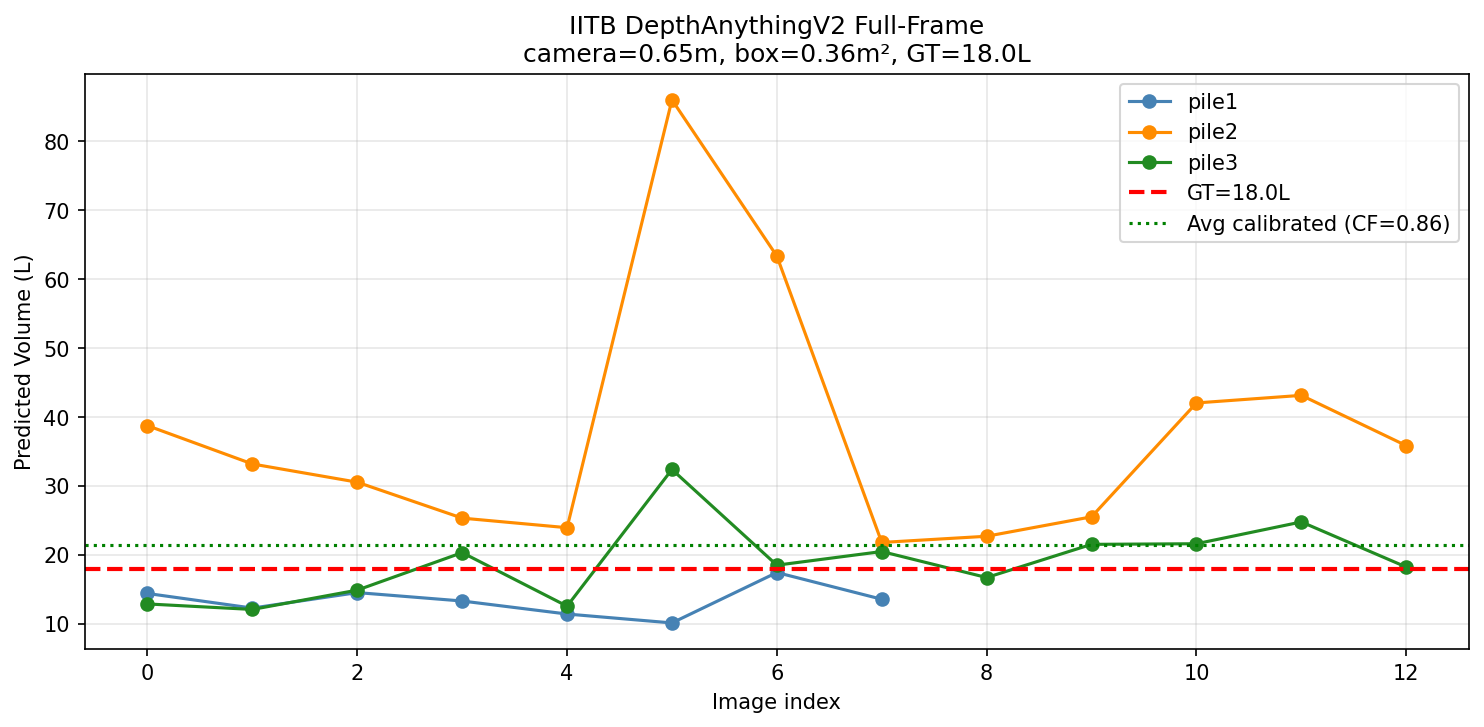
\includegraphics[width=0.82\linewidth]{images/volume_chart.png}
    \caption{Per-image raw volume predicti
    ons across all captures. The \textbf{x-axis} is
    the image index — each point represents one overhead photograph in the order it was
    processed; it has no temporal or spatial meaning and simply labels individual captures
    within each pile's dataset. The \textbf{dashed red line} marks the geometric ground-truth
    of 18~L. Pile~A (indices 0--N\textsubscript{A}) shows the tightest spread (CV = 15.6\%);
    Pile~B shows high variance partly due to anomalous captures with camera tilt or specular
    reflections (see Section~\ref{sec:discuss}); Pile~C clusters near 18~L with moderate
    spread.}
    \label{fig:chart}
\end{figure}

\subsection{Depth Sanity Verification}

A depth sanity check (centre depth smaller than edge-strip depth) was evaluated on every
captured image. All captures pass this check, with a mean centre-to-edge depth difference
of 6.5~cm for Pile A, 6.9~cm for Pile B, and 4.1~cm for Pile C (in scaled physical units).
This confirms that the depth model correctly identifies the pile as a raised surface in every
case.

% ==============================================================================
\section{Discussion}
\label{sec:discuss}

\subsection{Pile A: Consistent Underestimation Corrected by CF}

For the 670~g pile, the model consistently predicts a raw volume of approximately 13~L
(CV = 15.6\%). The calibration factor of 1.38 corrects this to 18.5~L, within 2.8\% of GT.
The underestimation arises because DepthAnythingV2 is calibrated to indoor scenes at 1--5~m
range; at 65~cm the depth variation across the pile spans a narrow portion of the model's
output range, resulting in compressed height estimates.

\subsection{Pile B: High Variance and GT Uncertainty}

Pile B (480~g) shows the highest raw variance (CV = 46.9\%) and a mean raw prediction of
37.8~L, more than twice the GT. Two captures exhibit anomalously high predicted volumes
(up to 87~L), likely due to camera tilt or specular reflectance from smooth surfaces in
the mixed-waste pile that caused the depth model to misinterpret near-field material.
Excluding these captures, the remaining Pile~B images average 27.5~L.

There is also reason to question the fixed geometric GT (18~L) for all three conditions:
a lighter, fluffier pile of mixed materials can occupy variable bulk volume depending on
how it is arranged. Displacement-based measurement is recommended to resolve this ambiguity.

\subsection{Pile C: Near-Unity CF, Good Accuracy}

For the 660~g pile, the raw mean prediction of 19.0~L requires only a CF of 1.02, meaning
the model already predicts close to GT without correction. The 7.8\% post-calibration
error (19.4~L vs.\ 18.0~L) likely reflects genuine pile-arrangement variation rather than
a model failure.

\subsection{Implications for Calibration Transfer}

The per-pile CFs range from 0.48 to 1.38, a factor of nearly 3. This large spread indicates
that a single global CF is not reliable across different pile masses or arrangements. For
practical deployment, a calibration set covering the expected range of pile sizes and material
types should be collected for each new site, with a recommended minimum of several GT-labelled
captures per condition.

% ==============================================================================
\section{Conclusion}
\label{sec:conclusion}

DepthAnythingV2-Metric-Indoor-Large, combined with floor-plane fitting and a one-parameter
calibration factor, estimates mixed solid-waste pile volumes from a single overhead RGB image
with errors below 8\% on two of three tested conditions. All captures pass the depth sanity
check. Raw predictions require per-condition calibration (CF ranges 0.48--1.38); a global CF
is insufficient. Ground-truth quality is the main remaining uncertainty: displacement-based
measurements are needed to replace the current geometric bounding-box estimate.

\subsection*{Next Evaluation Steps}

\begin{itemize}[leftmargin=1.5em,topsep=2pt,itemsep=1pt]
    \item Collect displacement- or water-based GT volumes for all pile conditions to remove
    bounding-box GT uncertainty.
    \item Expand the dataset to more pile mass levels and repeated arrangements to quantify
    CF stability within the same waste composition.
    \item Test calibration transfer across sites (different cameras, heights, and lighting) to
    assess how many GT-labelled captures are needed per new deployment.
    \item Evaluate whether a VLA (Vision-Language-Action) model can predict volume directly
    from image features, removing the need for per-condition calibration altogether.
\end{itemize}

% ==============================================================================
\section*{Acknowledgements}

Thank you to Praneel sir from PHO, for the on-site support for data collection

% ==============================================================================
\begin{thebibliography}{9}

\bibitem{depth_anything_v2}
L.~Yang, B.~Kang, Z.~Huang, X.~Xu, J.~Feng, and H.~Zhao,
``Depth Anything V2,''
\textit{Advances in Neural Information Processing Systems}, vol.~37, 2024.

\bibitem{sam}
A.~Kirillov et~al.,
``Segment Anything,''
\textit{Proceedings of the IEEE/CVF International Conference on Computer Vision}, 2023.

\bibitem{dino}
M.~Oquab et~al.,
``DINOv2: Learning Robust Visual Features without Supervision,''
\textit{Transactions on Machine Learning Research}, 2023.

\end{thebibliography}

\end{document}

